\chapter{Tune for the Primordial $k_T$}
\label{chap:primordialkTtune}

The primordial $k_T$ is another important parameter in the description of the proton-proton collisions with Monte Carlo simulations. The primordial $k_T$ description in \textsc{pythia8} was introduced in \secRef{sec:Beam Beam Remnants and primordial kT}.
\\
The main unresolved problem for the primordial $k_T$ tune is the unexpected high value required for the description of the observed $Z$ boson $p_T$ spectrum.
\\
In fact, the primordial $k_T$ found is origin in the Fermi Motion of the partons inside the hadrons. So when the parton undergoes to the hard scattering it can already have an initial no zero transverse momentum.
The value of the primordial $k_T$ can be estimate as reported in \eqRef{eq:PrimordialKT}, but in the case of the $Z$ boson $p_T$ spectrum this estimation is not sufficient the required value observed in order to reproduce the experimental data are in the order of $2\ \mathrm{GeV}$.

%The introduction of the primordial $k_T$ is really important in the description of the $Z$ boson $p_T$ spectrum. At the LO calculation there is nothing that can recoil against the $Z$ boson so it can only be produced with zero $p_T$. With the introduction of the primordial $k_T$ one have that the already at the LO the $Z$ can have a non zero primordial $k_T$.

So the introduction of the tune for the primordial $k_T$ is needed. In fact the CP5 tune it is known that does not describe well the $Z$ spectrum in the low-$p_T$ region \cite{CPtunes}. This is shown in \figRef{fig:CP5_notdescribeZjet} for the production cross-section in $Z$ plus jets events and in the figure \figRef{fig:CP5_notdescribeZ} for $Z$ boson production in DY observations. As we can se the CP5 tune is very far from experimental data values in the low regions. 

The distribution for $Z+$jets events as a function of the variable $p_T^{bal}=\big|p_T^Z-\sum_{\text{jets}}p_T^{j}\big|$ is not well described in the first bin. While the one as a function of the $p_T^Z$ miss the description in the region $p_T^Z \lesssim 40\ \mathrm{GeV}$. This two observable as described in \cite{CPtunes} are very sensitive to the parton shower process and UE.

For the tune we focus on the distribution in \figRef{fig:CP5_notdescribeZ} distributions, also here we can see that CP5 tune don't describe very well the low regions for this two observables.  
 

\begin{figure}[!htb]
	\centering
	\noindent
	\begin{subfigure}{0.5\textwidth}
		\centering
		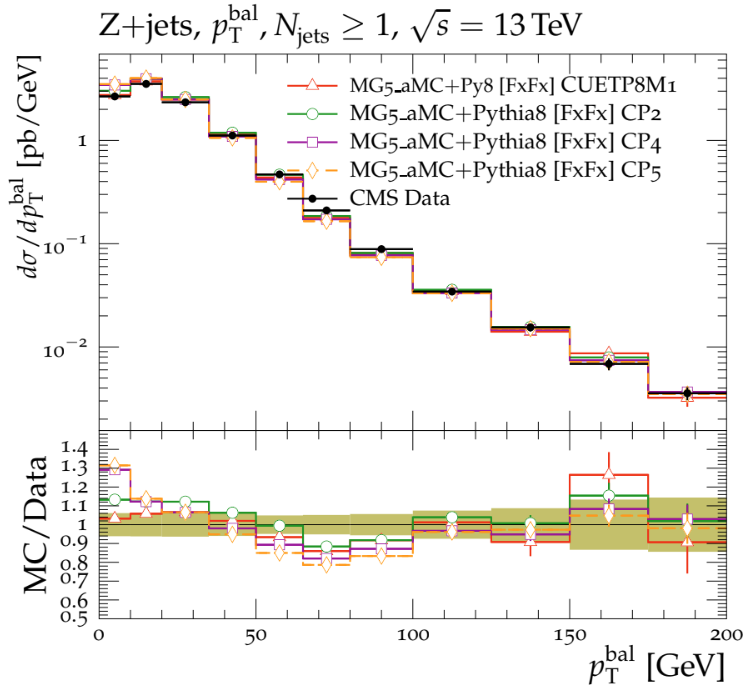
\includegraphics[width=0.985\textwidth]{{img/CPpaper_zjet1.png}}
	\end{subfigure}%
	\begin{subfigure}{0.5\textwidth}
		\centering
		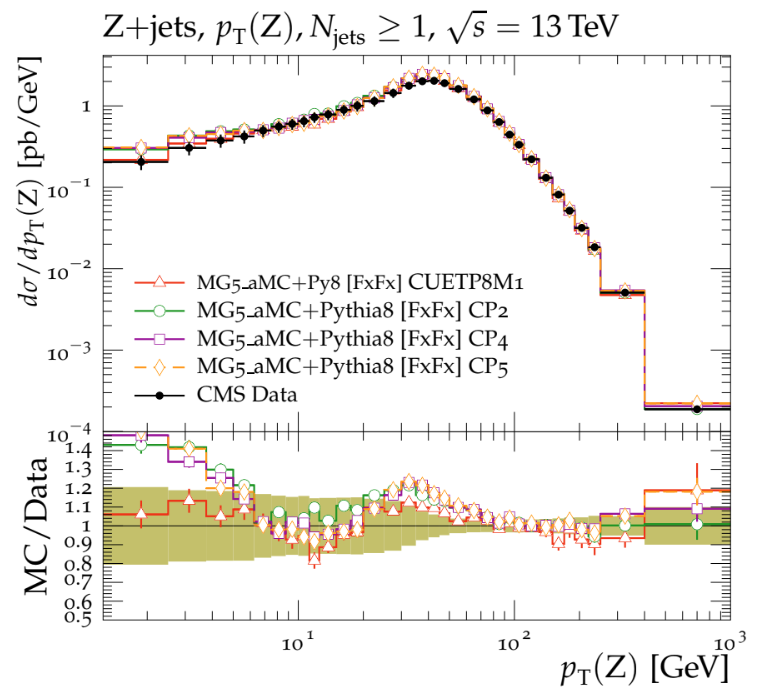
\includegraphics[width=\textwidth]{{img/CPpaper_zjet2.png}}
	\end{subfigure}%
	\caption{Figure from CP tunes presentation paper \cite{CPtunes}. These two images show the $Z$ boson production cross-section in $Z$ plus jets (with at least one jet) at $\sqrt{s}=13\ \mathrm{TeV}$ as a function of the imbalance of the transverse momentum between the jet and the $Z$ boson (left) and of the $Z$ boson transverse momentum (right) \cite{CMS:2018mdf}. The first bin in the left distribution and the regione $p_T^Z \lesssim 40\ \mathrm{GeV}$ in the right one are not well described by CP5 tune (yellow line).}
	\label{fig:CP5_notdescribeZjet}
\end{figure}

\begin{figure}[!htb]
	\centering
	\noindent
	\begin{subfigure}{0.5\textwidth}
		\centering
		\includegraphics[width=\textwidth]{{img/rivet-plots-PrimordialkT_only_CP5default/CMS_2019_I1753680/d27-x01-y03.pdf}}
	\end{subfigure}%
	\begin{subfigure}{0.5\textwidth}
		\centering
		\includegraphics[width=\textwidth]{{img/rivet-plots-PrimordialkT_only_CP5default/CMS_2019_I1753680/d28-x01-y03.pdf}}
	\end{subfigure}
	\caption{The CP5 tune is not good in the description of the low region of the $Z$ boson production cross-section of the $Z$ boson transverse momentum (left) or of the $\phi_\eta^*$ angle. This distribution are from the CMS analysis \cite{ZpT_distributions} at the center-of-mass energy of $13\ \mathrm{TeV}$.}
	\label{fig:CP5_notdescribeZ}
\end{figure}

\section{Primordial $k_T$ and ISR effect on $p_T^Z$}

The parameters on which we focus in order to tune data and explain the $Z$ boson $p_T$ spectrum are:
\begin{itemize}
\item \texttt{BeamRemnants:primordialKThard} that set the width of the Gaussian distribution for the primordial $k_T$ sample;
\item \texttt{SpaceShower:pT0Ref} that set the threshold for the initial state radiation to take place.
\end{itemize}
Let's see how this parameter impact on the $Z$ boson production. If we consider only the LO diagram for the $Z$ production we can have only a production with a zero transverse momentum. So the $Z$ spectrum we expect at LO is a $\delta$-distribution function.  

\begin{figure}[!htb]
	\centering
	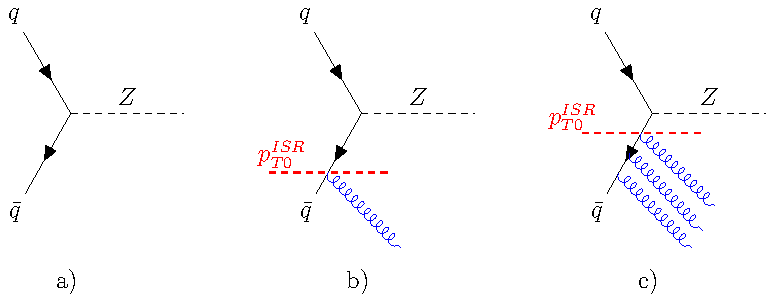
\includegraphics[width=0.8\textwidth]{{img/feynman_ZpT_2_blue.pdf}}
\end{figure}

With the addition of the primordial $k_T$ we get a Gaussian distribution which width is set by \texttt{BeamRemnants:primordialKThard}.
If we move to higher order diagrams the $Z$ boson can be produced with a non zero $p_T$ that is balanced by the various jets, then the primordial $k_T$ is added to the already non-zero $Z$ boson transverse momentum. 

A large contribution come also from the amount of ISR that is emitted from the incoming partons, in fact each split can give to the incoming parton a non-zero initial value of $p_T$ and so the $Z$ boson is created with a non-zero $p_T$ before the introduction of the primordial $k_T$. 

An higher amount of ISR, so a lower value for the threshold, can lead to a larger $p_T$ taken from the parton that generate the $Z$ boson with an higher $p_T$ and vice versa.

\section{Primordial $k_T$ tune}

The primordial $k_T$ was not investigated by CP5 so it is important to include that in the analysis in order to describe better the low $p_T$ region. 

The parameters variation ranges we use are the one reported in the \tableRef{table:primordialkT_variations} while others parameters are set to CP5 values.



\begin{table}[!htb]
\centering
\begin{tabular}{l | c }
Parameter Name & Value \\ 
\hline \hline
\\[-0.85em]
	\texttt{BeamRemnants:primordialKThard} & $[0.5 - 5.0]$\\[2pt]
	\texttt{SpaceShower:pT0Ref} & $[0.5 - 5.0]$\\
\end{tabular}
\caption{Variation ranges for the sampling used in the primordial $k_T$ tune.}
\label{table:primordialkT_variations}
\end{table} 

The number of samples is lower than the one used for the Underlying Event in fact the training set we use for the PerBin Model contains more or less $160$ MC runs and a little more for the Inverse Model, $\sim 200$.

\figRef{fig:CP5_notdescribeZ} shows the distributions used to performed the tune. The distributions  are from the \cite{ZpT_distributions} analysis at $\sqrt{s}=13\ \mathrm{TeV}$:
\begin{itemize}
	\item The $Z$ boson production cross-section in DY observation as a function of $p_T^Z$;
	\item The $Z$ boson production cross-section in DY observation as a function of $\phi_\eta^*$.
\end{itemize}

 
\begin{figure}[!htb]
	\centering
	\noindent
	\begin{subfigure}{0.48\textwidth}
	\centering
	\includegraphics[width=\textwidth]{{img/rivet-plots-PrimordialkT_PerBin_vs_Inverse_vs_CP5_FxFx_weights/CMS_2019_I1753680/d27-x01-y03.pdf}}	
	\end{subfigure}%
	\begin{subfigure}{0.48\textwidth}
	\centering
	\includegraphics[width=\textwidth]{{img/rivet-plots-PrimordialkT_PerBin_vs_Inverse_vs_CP5_FxFx_weights/CMS_2019_I1753680/d28-x01-y03.pdf}}	
	\end{subfigure}
\end{figure}

\begin{figure}[!htb]
	\centering
	\noindent
	\begin{subfigure}{0.48\textwidth}
	\centering
	\includegraphics[width=\textwidth]{{img/rivet-plots-PrimordialkT_PerBin_vs_Inverse_vs_CP5_FxFx_noWeights/CMS_2019_I1753680/d27-x01-y03.pdf}}	
	\end{subfigure}%
	\begin{subfigure}{0.48\textwidth}
	\centering
	\includegraphics[width=\textwidth]{{img/rivet-plots-PrimordialkT_PerBin_vs_Inverse_vs_CP5_FxFx_noWeights/CMS_2019_I1753680/d28-x01-y03.pdf}}	
	\end{subfigure}
\end{figure}


